\providecommand{\pdfxopt}{a-1b,mathxmp}

% \documentclass[10pt]{article}
% \usepackage{beamerarticle}
\documentclass[ignorenonframetext,aspectratio=169]{beamer}

\input{/home/asreeve/current/class/ers102/pre_latex/luatex_pre.tex}
\usepackage{cancel}

\setbeamertemplate{enumerate item}[square]
\setbeamertemplate{enumerate subitem}[circle]
\setbeamertemplate{enumerate subsubitem}[square]
\setbeamercolor*{enumerate item}{fg=red,bg=blue}
\setbeamercolor*{enumerate subitem}{fg=blue,bg=red}

\begin{document}

\begin{frame}{Topographic Maps \tiny Bottom half of Princeton ME 7.5 minute quad}
  \begin{minipage}{.7\textwidth}
    \begin{center}
      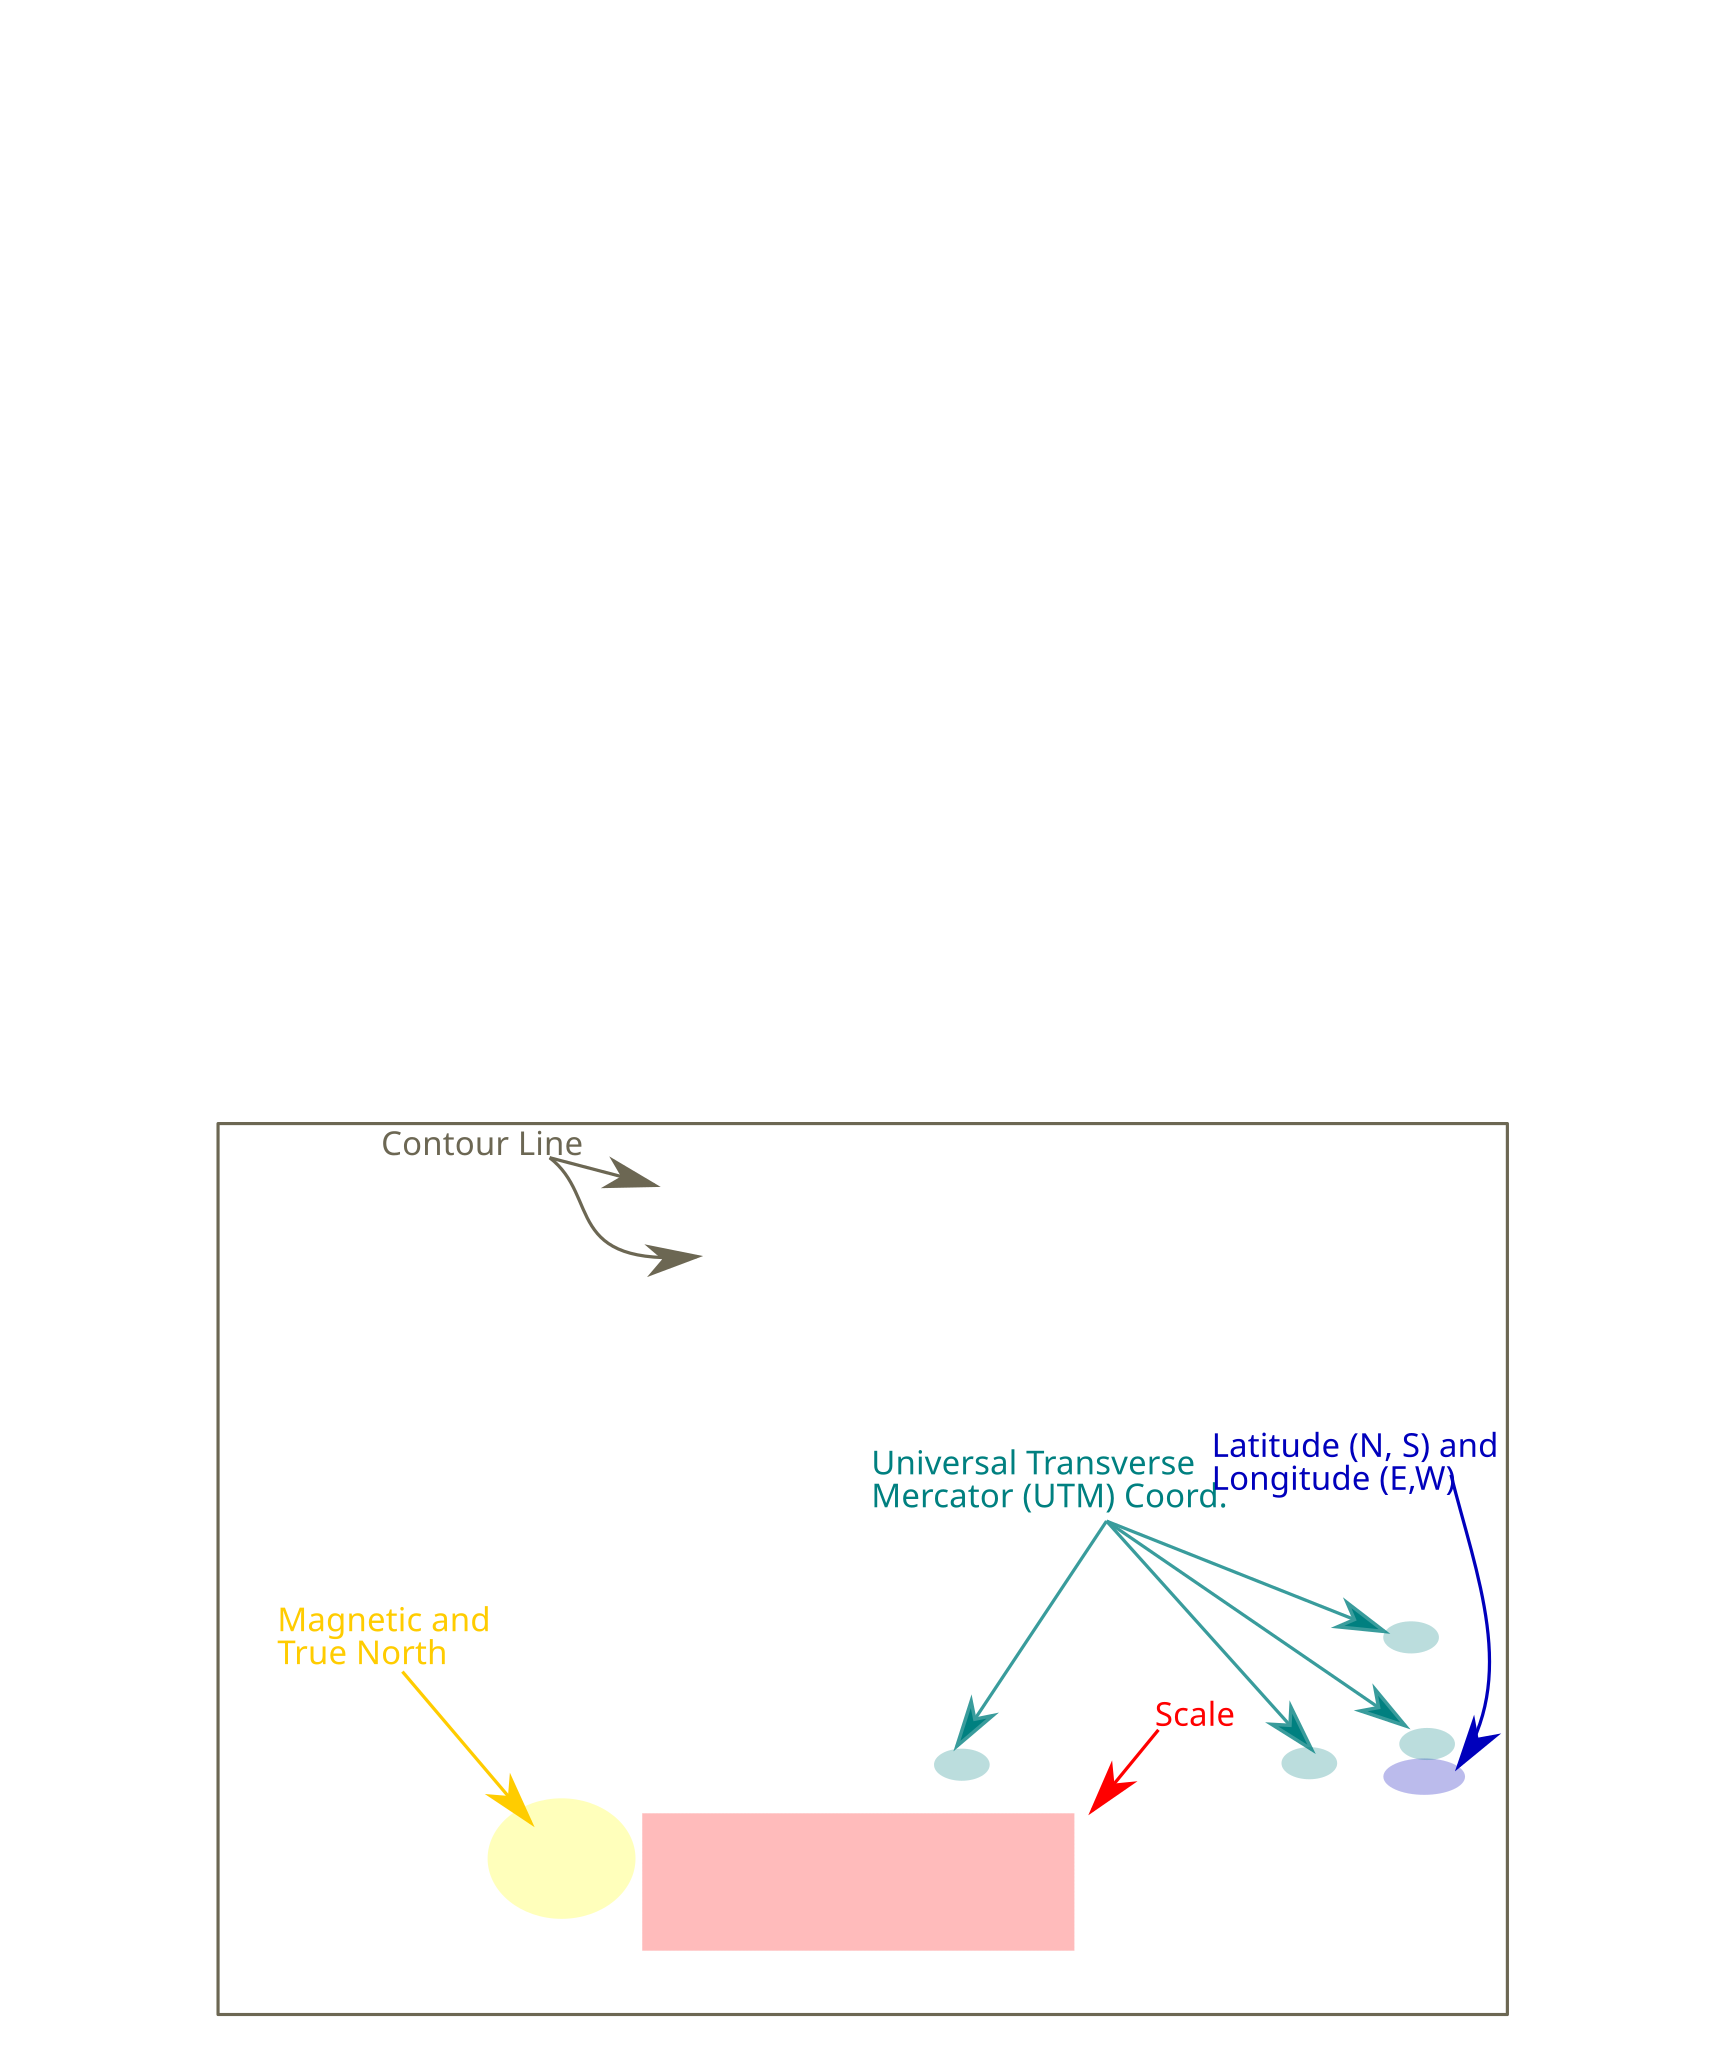
\includegraphics[width=\textwidth]{./Topo_Info.png}
    \end{center}
  \end{minipage}
  \begin{minipage}{.28\textwidth}
    2-D depiction of 3-D land surface
    \begin{enumerate}
    \item Contour lines: line of equal elevation
    \item Cultural features: house/roads/water/etc.
    \item Scale: distances on map
    \item Geographic Location (Lat \& Long)
    \end{enumerate}
  \end{minipage}
\end{frame}

\begin{frame}{Scale}
  \begin{minipage}{.4\textwidth}
    \begin{center}
      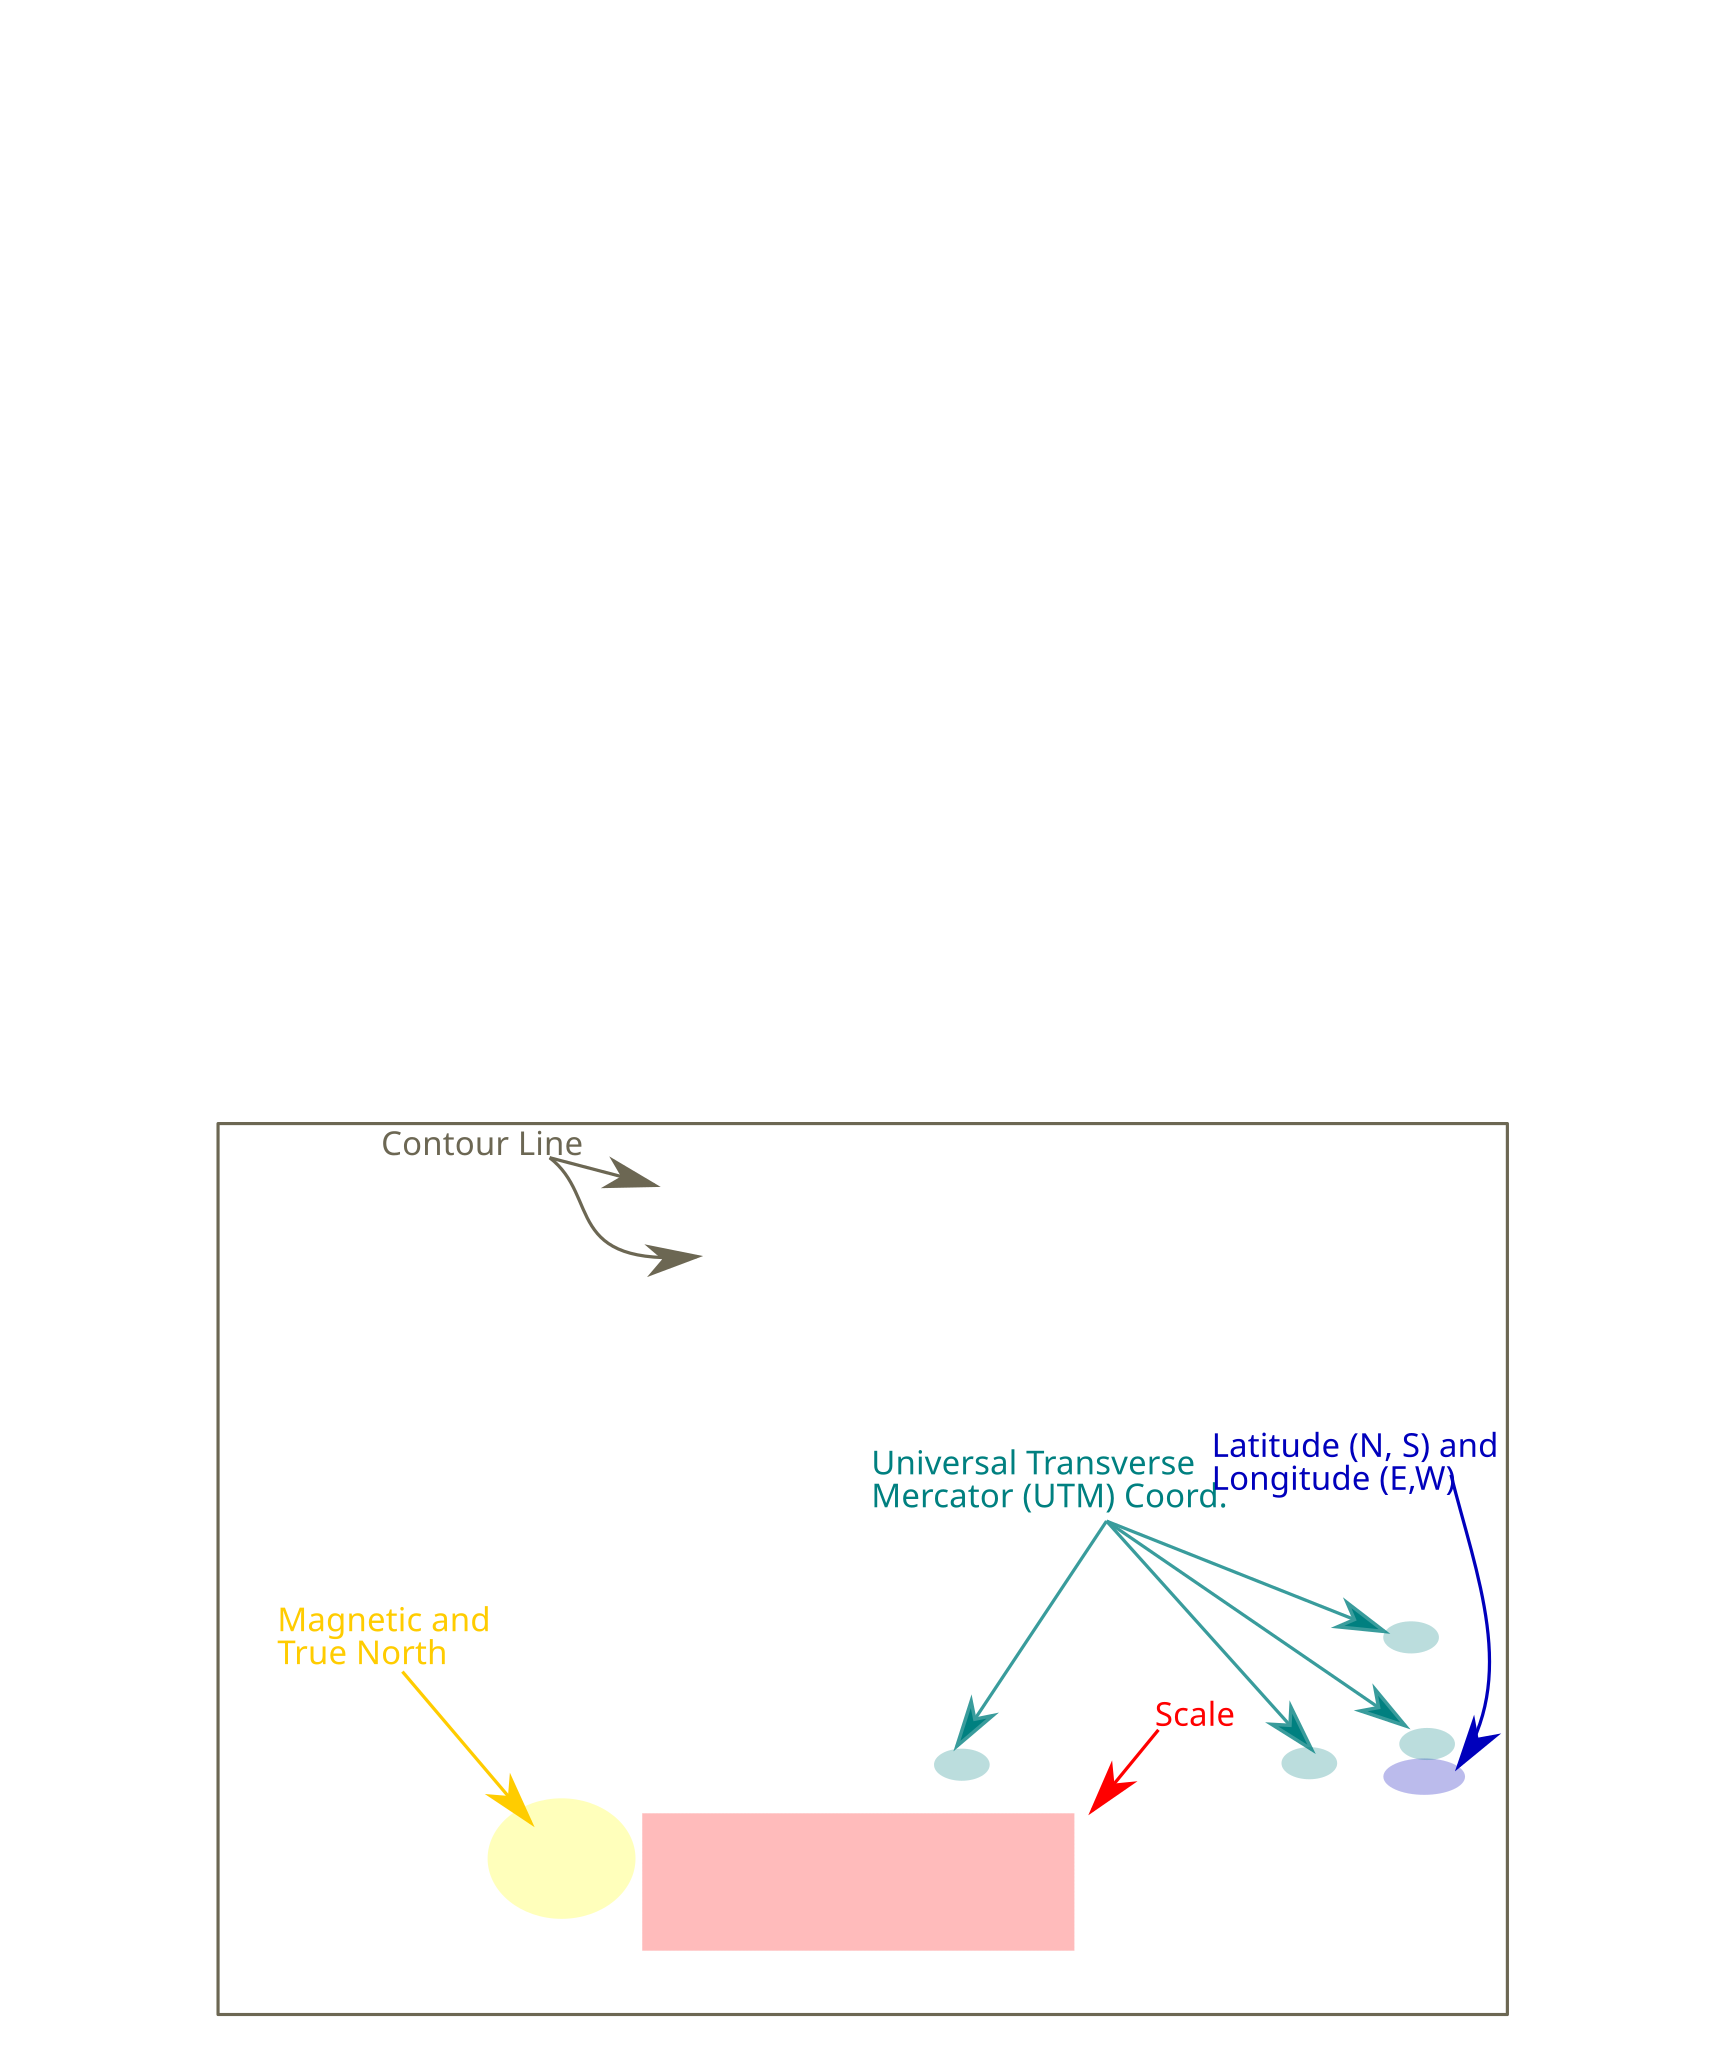
\includegraphics[width=\textwidth]{./Topo_Info.png}
    \end{center}
  \end{minipage}
  \begin{minipage}{.58\textwidth}
    \begin{description}
    \item[Graphical] Bar with real world length indicated 
    \item[Verbal] Statement (e.g. 'one centimeter represents 1 km')
    \item[Ratio] a fraction, e.g 1:2000, map distance to real world distance
    \end{description}
  \end{minipage}
  \small
  If the scale on the map is '1:20000', means 1 cm on map equals 20000 cm in reality or 1 map inch equals 20000 real inches or ...

  I don't know how far 2000 inches is in km, need to convert, multiply by fractions where top and bottom are the same length expressed in different units.

  \begin{equation*}
    \underbrace{20000 \; \cancel{inch}}_{starting \; value} \times \frac{2.54 \; \bcancel{cm}}{1 \; \cancel{inch}} \times
    \frac{1 \; \xcancel{m}}{100 \; \bcancel{cm}} \times \frac{1 \; km}{1000 \; \xcancel{m}}
    = 0.51 \; km
  \end{equation*}
\end{frame}

\begin{frame}{Geographic location}
  \begin{minipage}{.5\textwidth}
    \begin{center}
      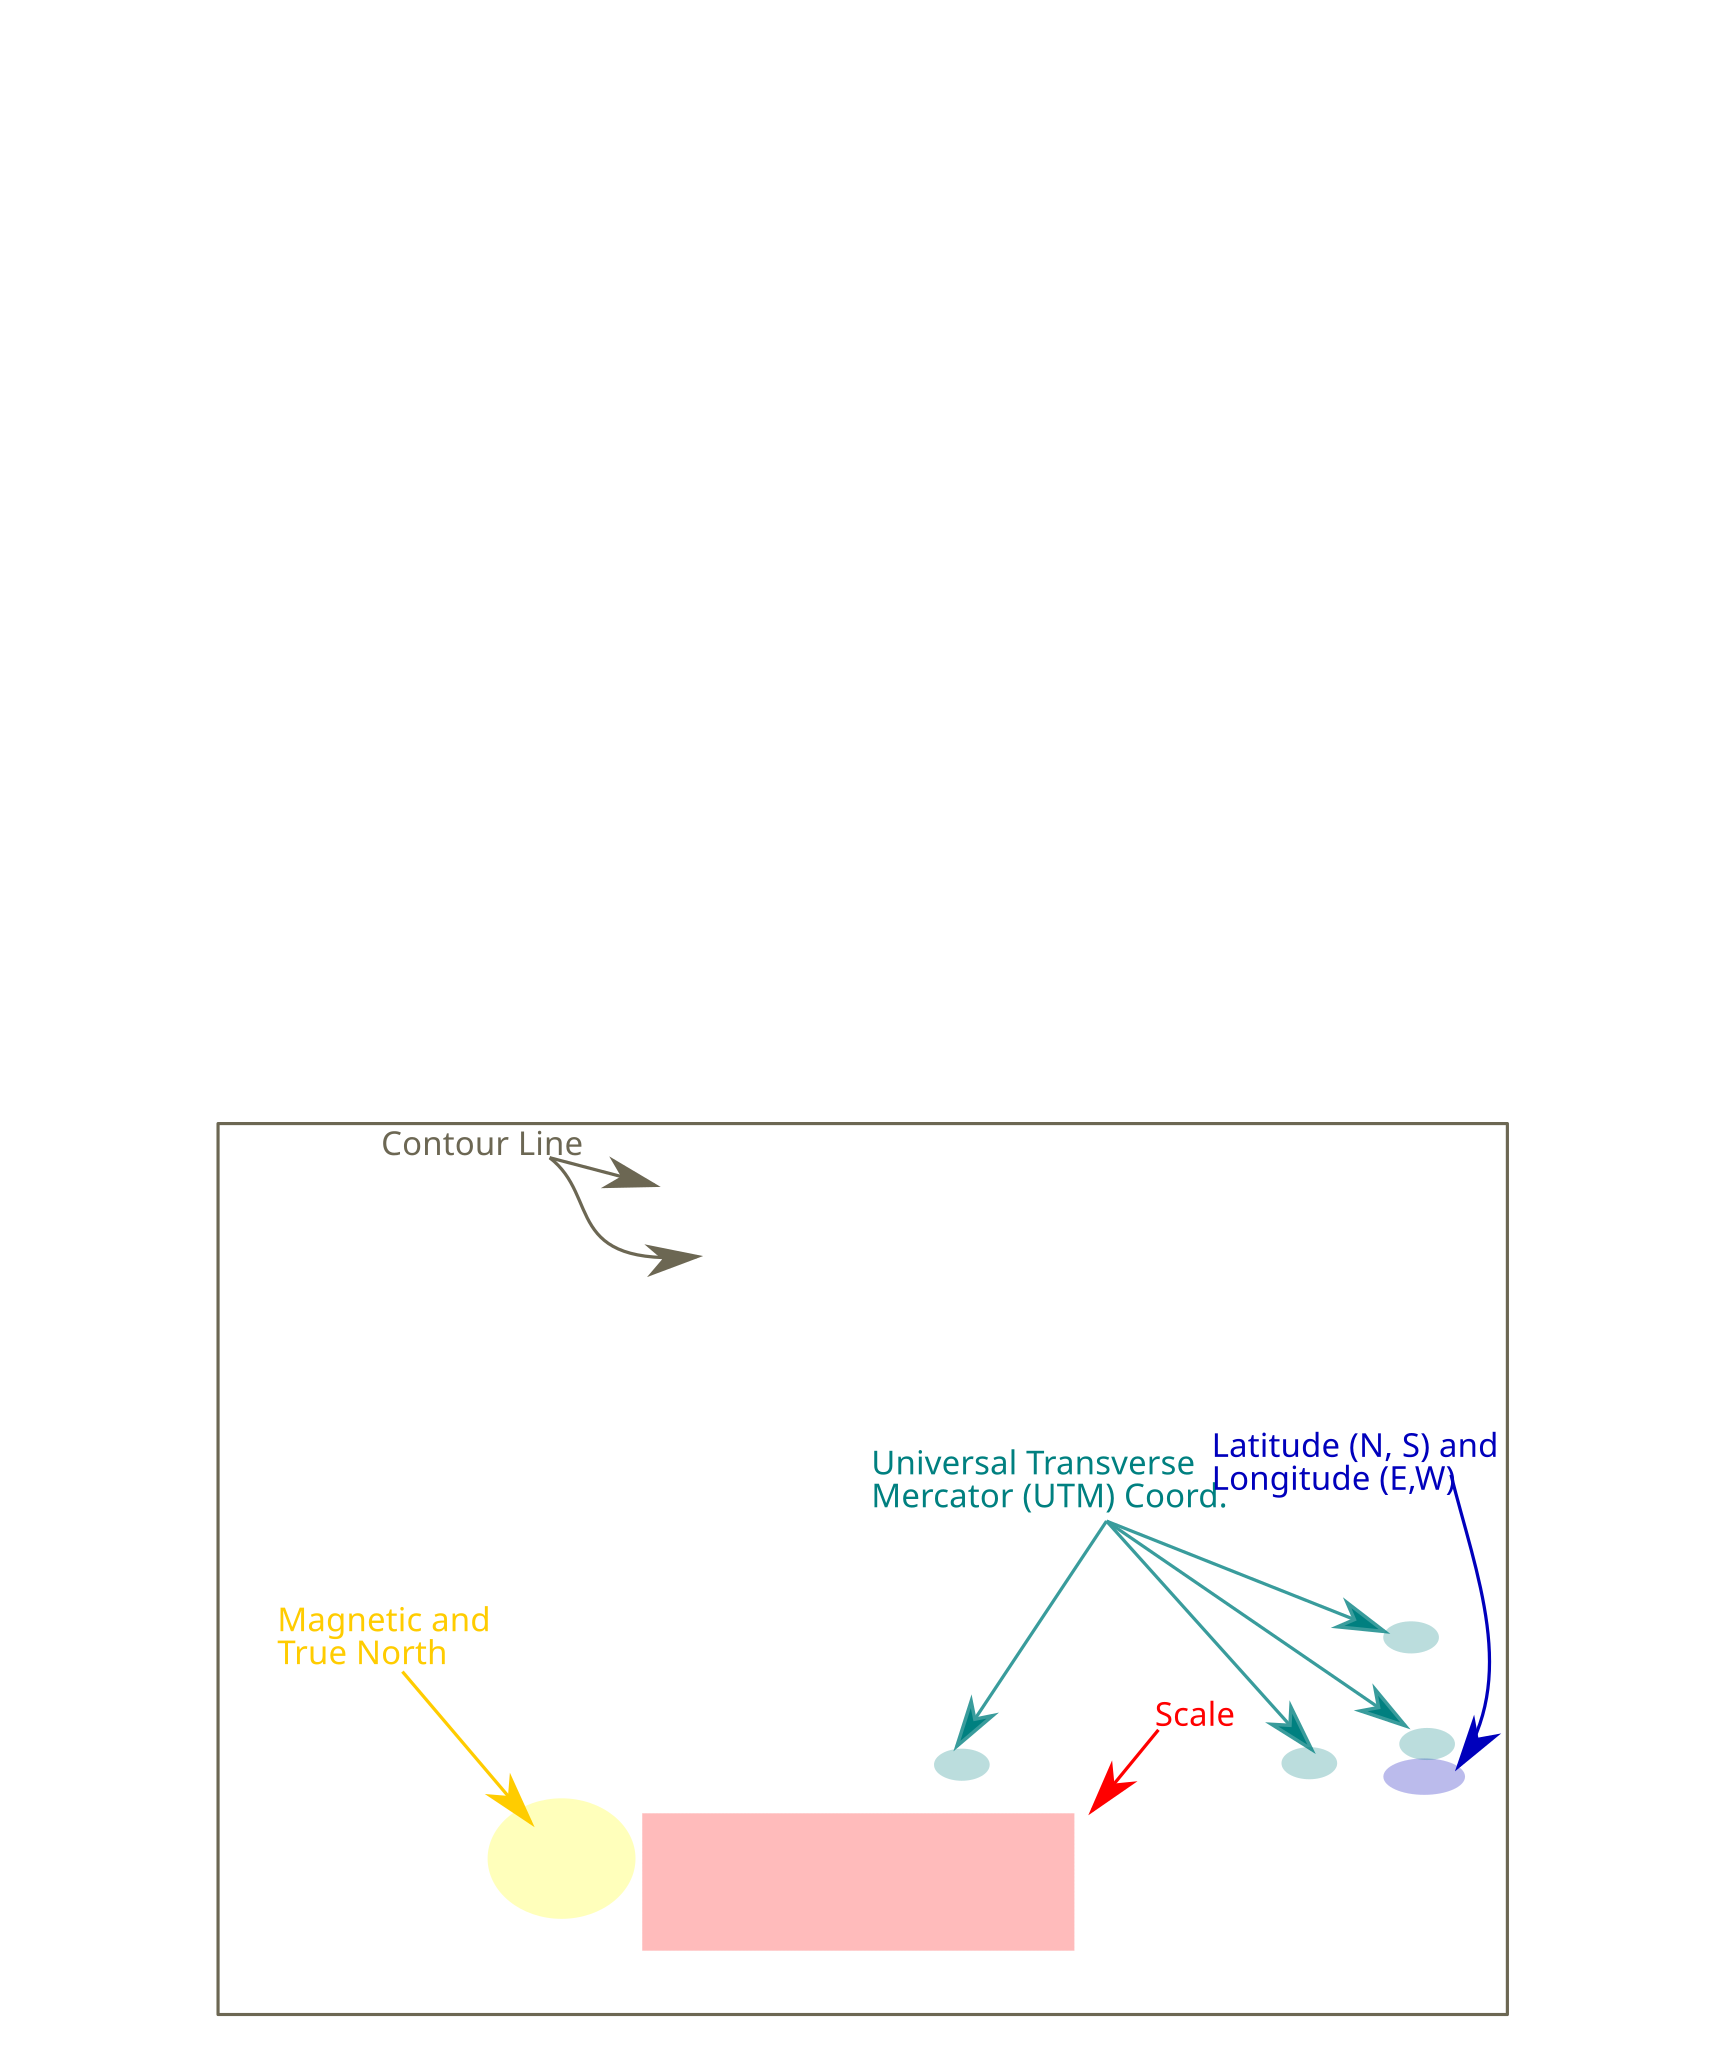
\includegraphics[width=\textwidth]{./Topo_Info.png}
    \end{center}
  \end{minipage}
  \begin{minipage}{.48\textwidth}
    \begin{description}
    \item[UTM] Breaks up world in grid, uses metric system to indicate distance in meters N and E of a point on the globe \tiny (N from equator (for Northern Hemisphere) and E from central meridian with value of 500,000 m) \normalsize
    \item[Latitude \& Longitude] Angular position; origin is Equator and Prime (Greenwich, England) Meridian; seconds$^{''}$, minutes$^{'}$ and degrees$^{\circ}$.
    \item[State Plane] distance (ft) from reference lines in each state, only in USA, obsolete
    \end{description}
  \end{minipage}
\end{frame}

\begin{frame}{Contour Lines}
  \begin{minipage}{.4\textwidth}
    \begin{center}
      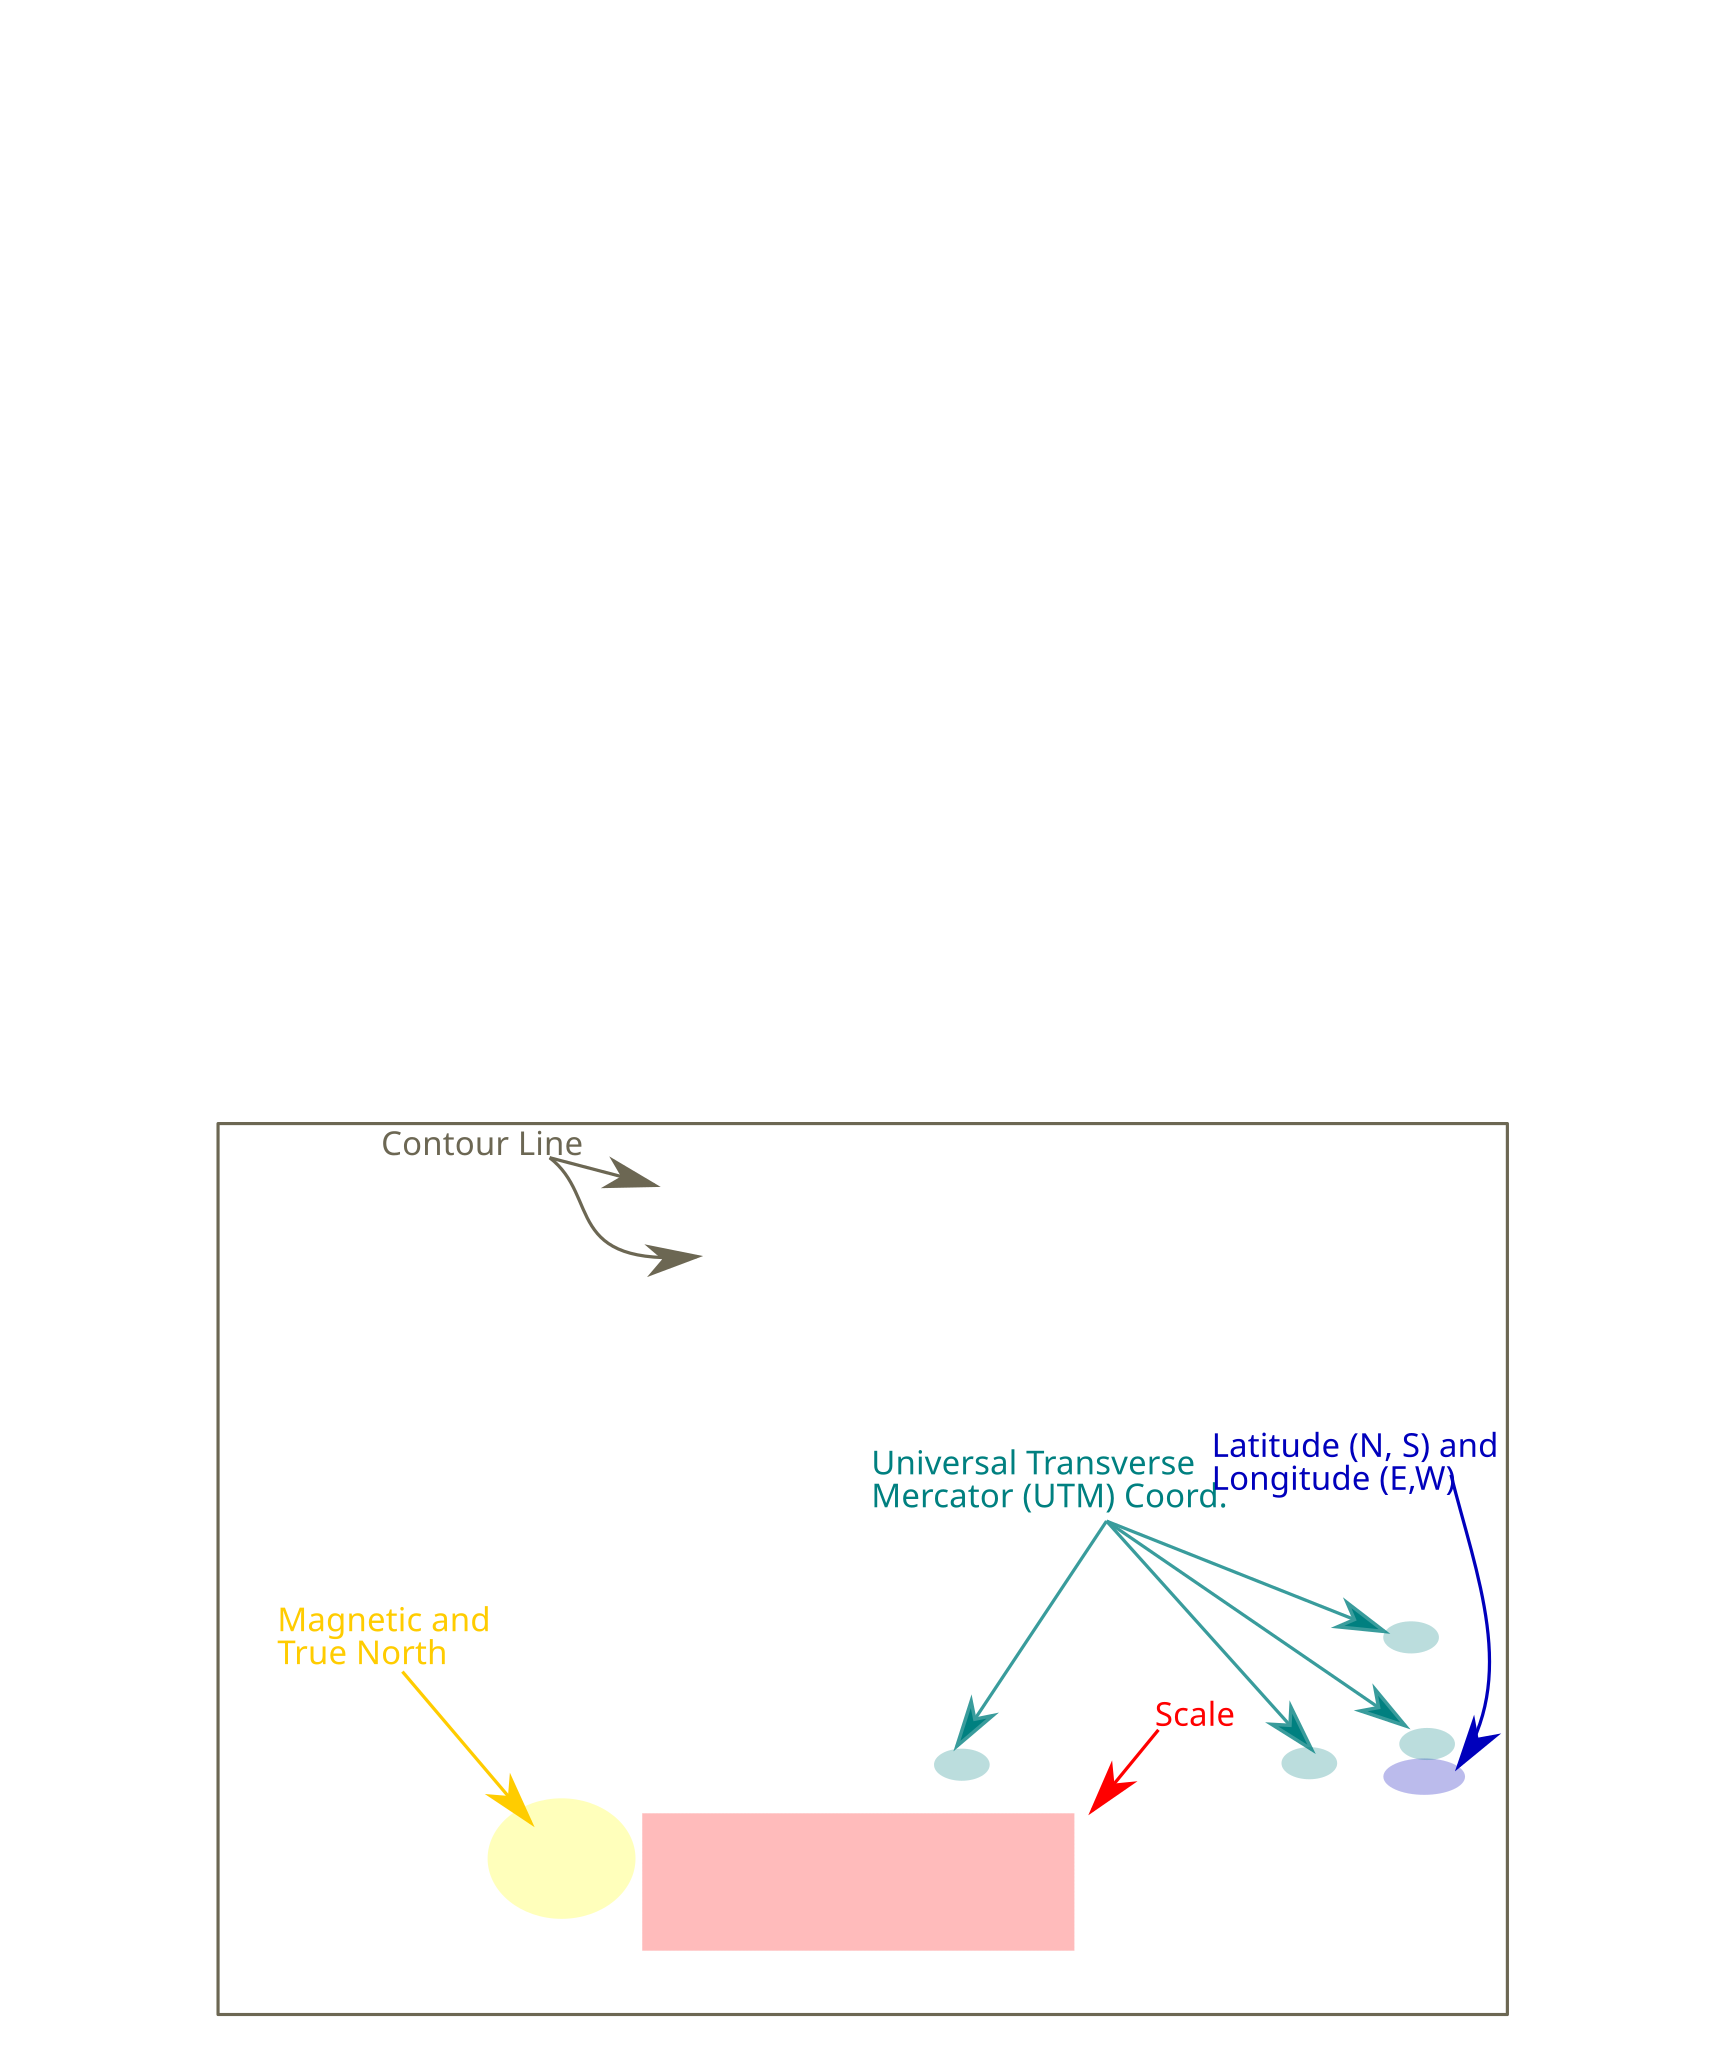
\includegraphics[width=\textwidth]{./Topo_Info.png}
    \end{center}
  \end{minipage}
  \begin{minipage}{.58\textwidth}
  \begin{enumerate}
    \item contour lines represent locations of equal elevation on a map
    \item contour interval is vertical spacing between (lighter) lines on map
    \item Rules
      \begin{itemize}
      \item don't touch or split
      \item close or exit map
      \item 'v' across 'channels', pointing upstream
      \end{itemize}
    \end{enumerate}
  \end{minipage}    
\end{frame}
\begin{frame}{Contour Lines}
    \begin{minipage}{.4\textwidth}
    \begin{center}
      \includegraphics<1>[width=\textwidth]{./Contour_example1.pdf}
      \includegraphics<2>[width=\textwidth]{./Contour_example2.pdf}
      \includegraphics<3>[width=\textwidth]{./Contour_example3.pdf}
    \end{center}
  \end{minipage}
  \begin{minipage}{.58\textwidth}
    \begin{enumerate}
    \item contour lines represent locations of equal elevation on a map
    \item contour interval is vertical spacing between (lighter) lines on map
    \item Rules
      \begin{itemize}
      \item don't touch or split
      \item close or exit map
      \item 'v' across 'channels', pointing upstream
      \end{itemize}
    \end{enumerate}
  \end{minipage}    
\end{frame}
\end{document}
